% !TeX root = RJwrapper.tex
\title{Title of your article}
\author{by Author One and Author Two}

\maketitle

\abstract{%
An abstract of less than 150 words.
}

\hypertarget{introduction}{%
\section{Introduction}\label{introduction}}

Introductory section which may include references in parentheses
\citep{R}, or cite a reference such as \citet{R} in the text.

\hypertarget{section-title-in-sentence-case}{%
\subsection{Section title in sentence
case}\label{section-title-in-sentence-case}}

This section may contain a figure such as Figure \ref{fig:Rlogo}.

\begin{Schunk}
\begin{figure}[htbp]

{\centering 
\includegraphics[width=2in]{Rlogo-5} 

}

\caption[The logo of R]{The logo of R.}\label{fig:Rlogo}
\end{figure}
\end{Schunk}

\hypertarget{another-section}{%
\subsection{Another section}\label{another-section}}

There will likely be several sections, perhaps including the proposal of
a new package xyz, some codes and plots

\begin{Schunk}

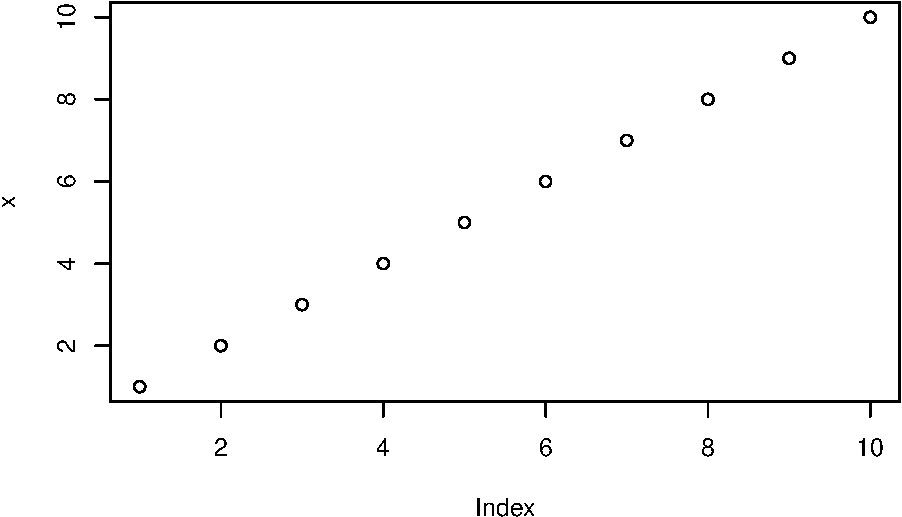
\includegraphics{sample-article_files/figure-latex/unnamed-chunk-1-1} \end{Schunk}

\hypertarget{summary}{%
\subsection{Summary}\label{summary}}

This file is only a basic article template. For full details of
\emph{The R Journal} style and information on how to prepare your
article for submission, see the
\href{https://journal.r-project.org/share/author-guide.pdf}{Instructions
for Authors}.

\bibliography{sample-article.bib}

\address{%
Author One\\
Affiliation\\%
line 1\\ line 2\\
%
\url{https://journal.r-project.org}%
\\\textit{ORCiD: \href{https://orcid.org/0000-0002-9079-593X}{0000-0002-9079-593X}}%
\\\href{mailto:author1@work}{\nolinkurl{author1@work}}
}

\address{%
Author Two\\
Affiliation 1\\%
line 1 affiliation 1\\ line 2 affiliation 1\\
Affiliation 2\\%
line 1 affiliation 2\\ line 2 affiliation 2\\
%
\url{https://journal.r-project.org}%
\\\textit{ORCiD: \href{https://orcid.org/0000-0002-9079-593X}{0000-0002-9079-593X}}%
\\\href{mailto:author2@work}{\nolinkurl{author2@work}}
}
